\documentclass[a4paper, 12pt]{article}%тип документа

%отступы
\usepackage[left=2cm,right=2cm,top=2cm,bottom=3cm,bindingoffset=0cm]{geometry}

%Русский язык
\usepackage[T2A]{fontenc} %кодировка
\usepackage[utf8]{inputenc} %кодировка исходного кода
\usepackage[english,russian]{babel} %локализация и переносы

%Вставка картинок
\usepackage{wrapfig}
\usepackage{graphicx}
\graphicspath{{pictures/}}
\DeclareGraphicsExtensions{.pdf,.png,.jpg}

%оглавление
\usepackage{titlesec}
\titlespacing{\chapter}{0pt}{-30pt}{12pt}
\titlespacing{\section}{\parindent}{5mm}{5mm}
\titlespacing{\subsection}{\parindent}{5mm}{5mm}
\usepackage{setspace}

%Графики
\usepackage{multirow}
\usepackage{pgfplots}
\pgfplotsset{compat=1.9}

%Математика
\usepackage{amsmath, amsfonts, amssymb, amsthm, mathtools}

%Стиль страницы
\usepackage{fancyhdr}
\pagestyle{fancy}

\begin{document}

\begin{titlepage}

\begin{center}
%\vspace*{1cm}
\large\textbf{Московский Физико-Технический Институт}\\
\large\textbf{(государственный университет)}
\vfill
\line(1,0){430}\\[1mm]
\huge\textbf{Работа 5.4.1}\\
\line(1,0){430}\\[1mm]
\vfill
\large Сибгатуллин Булат, ФРКТ\\
\end{center}

\end{titlepage}
\fancyhead[L] {Работа 5.4.1.}
\noindent \textbf{Цель работы:} \\
\indent Измерить пробег альфа-частиц в воздухе двумя способами: с помощью торцевого счетчика Гейгера и ионизационной камеры.\\

\section{Теоретическое введение и описание установки}
	
	В качестве источника альфа-частиц используется $ ^{239}  $Pu  с периодом полураспада $ T_{1/2} = 2,44 \cdot 10^4 $ лет. Альфа-частицы, испускаемые $ ^{239} Pu $, состоят из трех моноэнергетических групп, различие между которы-
	ми лежит в пределах 50 кэВ. При той точности, которая достигается
	в наших опытах, их можно считать совпадающими по энергии, равной
	5,15 МэВ.
	
	\subsection{Счетчик Гейгера}
	
	\begin{wrapfigure}[15]{l}{0.25\linewidth}
		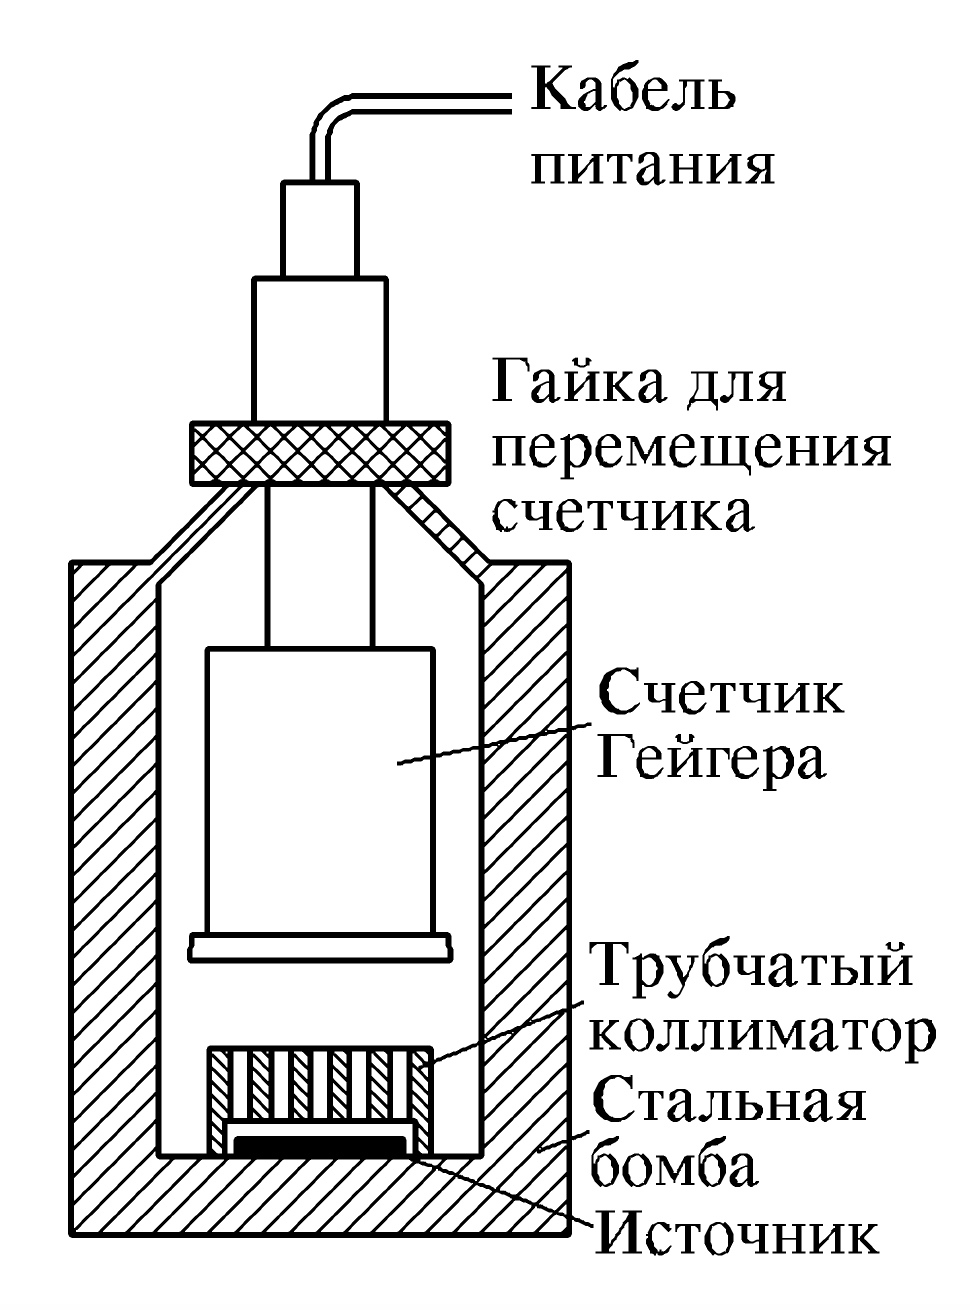
\includegraphics[width=\linewidth]{images/Geyger.jpg}
		\caption{Схема торцевого счетчика Гейгера}
		\label{ris geyger}
	\end{wrapfigure}
	
	Для определения пробега альфа-частиц с помощью счетчика радиоактивный источник помещается на дно стальной цилиндрической бомбы
	(рис. \ref{ris geyger}), в которой может перемещаться торцевой счетчик Гейгера. Его
	чувствительный объем отделен от наружной среды тонким слюдяным
	окошком, сквозь которое могут проходить альфа-частицы. Рабочее напря-
	жение счетчика указано на установке.
	
	Импульсы, возникающие в счетчике, усиливаются и регистрируются пересчетной схемой. Путь частиц в воздухе зависит от расстояния между источником и счетчиком. Перемещение счетчика производится путем вращения гайки, находящейся на крышке бомбы. Расстояние
	между счетчиком и препаратом измеряется по шкале, нанесенной на
	держатель счетчика. Счетчик не может быть придвинут к препарату ближе чем на 10 мм, т. к. между источником и счетчиком установлен коллиматор, изготовленный из плотно сжатых металлических трубок. Отверстия трубок пропускают к счетчику только те альфа-частицы, которые вылетают из источника почти перпендикулярно его поверхности.
	
	\subsection{Ионизационная камера}
	
	Ионизационная камера --- прибор для количественного измерения
	ионизации, произведенной заряженными частицами при прохождении
	через газ. Камера представляет собой наполненный газом сосуд с двумя электродами (схема камеры приведена на рис. \ref{ris Ion}). Сферическая стенка прибора служит одним из электродов, второй электрод вводится в газ через изолирующую пробку. К электродам подводится постоянное напряжение от источника ЭДС.
	
	Заполняющий сосуд газ сам по себе не проводит электрический ток, возникает он только при прохождении быстрой заряженной частицы, которая рождает в газе на своем пути ионы.
	
	Поместим на торец внутреннего электрода источник
	ионизирующего излучения (в нашем случае это источник
	альфа-частиц $ ^{239}_{94} $Pu), заполним объем камеры воздухом и начнем
	постепенно увеличивать разность потенциалов между электродами. Ток, протекающий через камеру, вначале будет резко возрастать, а затем, начиная с некоторого напряжения $ V_0 $, станет постоянным, т. е. "<выйдет на плато">.  Предельный ток $ I_0 $ будет равен $ I_0 = n_0e $,
	где $ n_0 $ --- число пар ионов, образуемых в секунду в объеме камеры, а $ e $ --- заряд электрона.
	
	\begin{wrapfigure}[16]{l}{0.37\linewidth}
		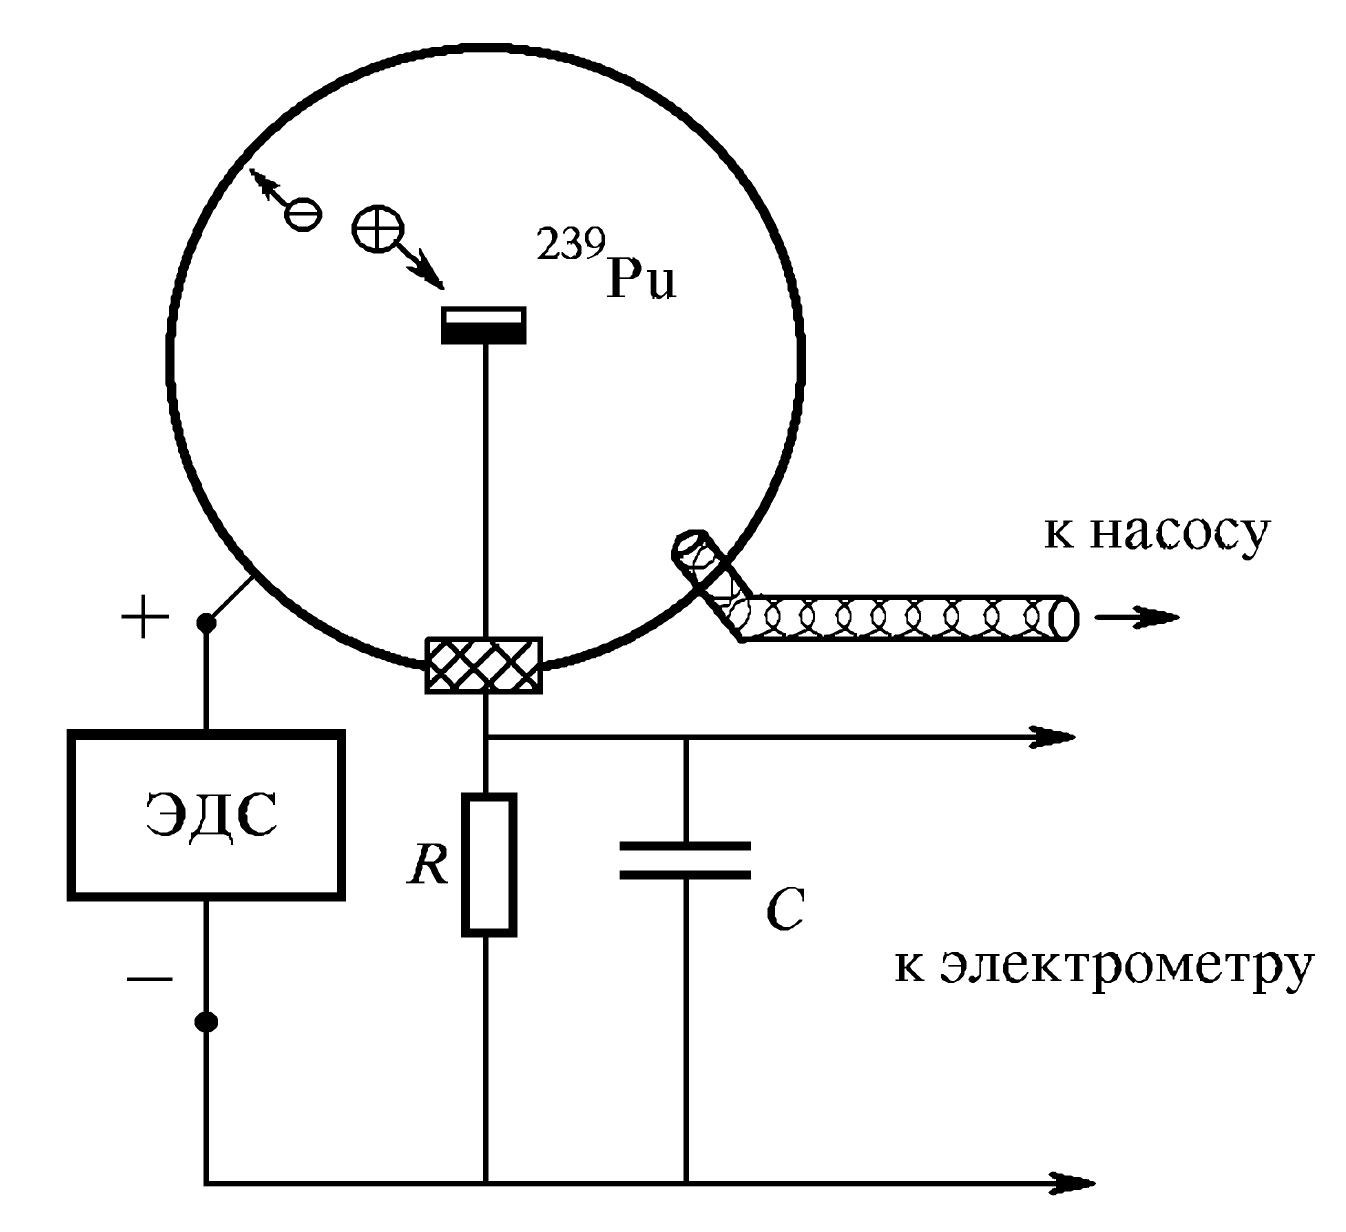
\includegraphics[width=\linewidth]{images/Ion.png}
		\caption{Схема устройства ионизационной камера}
		\label{ris Ion}
	\end{wrapfigure}
	
	Прохождение тока через камеру регистрируется посредством измерения напряжения на включенном в цепь камеры сопротивлении $ R $.
	Так как средняя энергия ионизации атомов воздуха составляет около 30 эВ, то альфа-частица с энергией 3 МэВ образует на своем пути около $ 10^5 $ электронов, им соответствует заряд $1,6 \cdot 10^{-14} $ Кл. Чтобы
	столь малое количество заряда, создаваемое проходящей через камеру одной альфа-частицей, вызывало измеряемое напряжение, емкость $ C $
	должна быть мала.
	
	Так как подвижность электронов примерно в 1000 раз больше подвижности ионов, то подбором параметров $ RC $-цепочки можно выделить импульсы тока, соответствующие только возникающей электронной компоненте. Реально регистрация электронной компоненты
	импульса тока обеспечивается при величине постоянной времени $ RC $-
	цепочки в несколько микросекунд.
	Если число проходящих через камеру альфа-частиц достаточно велико, то можно регистрировать не заряд, а величину возникающего тока, которая, естественно, пропорциональна интенсивности альфа-частиц. В
	токовом режиме величину постоянной времени $ RC $-цепочки устанавливают равной нескольким секундам, а работающую в этом режиме
	камеру называют токовой.
	
	\begin{wrapfigure}[15]{r}{0.3\linewidth}
		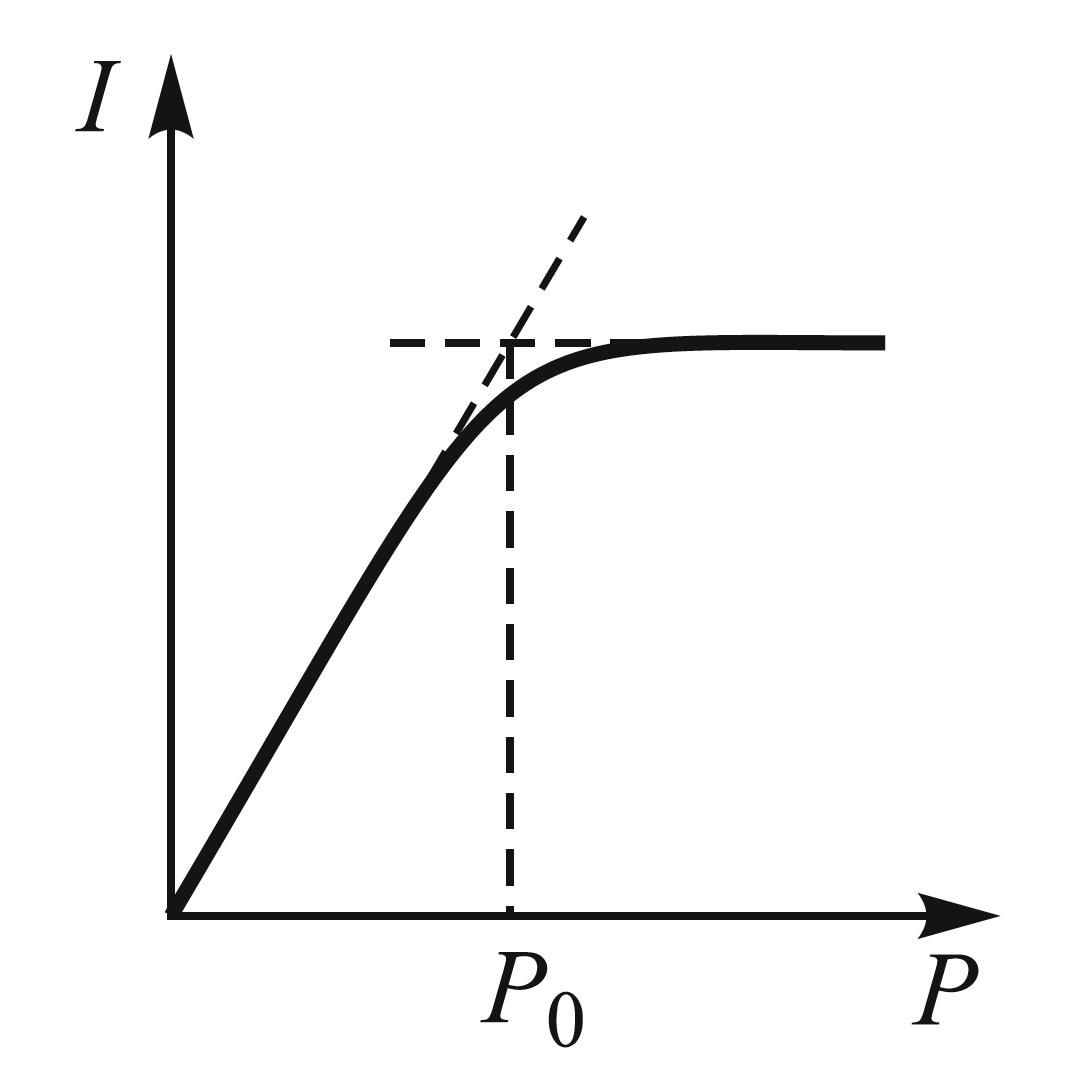
\includegraphics[width=\linewidth]{images/PotI.png}
		\caption{Характерная кривая зависимости
			тока ионизационной камеры от давления.
			Ионизация создается $ \alpha $-частицами}
		\label{ris PotI}
	\end{wrapfigure}
	
	При изменении давления в камере ионизационный ток меняется так, как это показано на рис. \ref{ris PotI}. При небольших давлениях газа
	альфа-частицы передают часть энергии стенкам камеры. По достижении
	давления $ P_0 $ все они заканчивают свой пробег внутри газа, и дальнейшее возрастание тока прекращается. Для определения давления $ P_0 $ чаще всего пользуются методом экстраполяции (полученная таким методом величина называется экстраполированным пробегом), продолжая наклонный и горизонтальный участки кривой до пересечения. Найденный таким образом пробег затем должен быть приведен к нормальному давлению и температуре $ 15 ^\circ C $.
	
	В данной работе измерение пробега альфа-частицы проводится по величине тока ионизации в сферической камере. Внутренним электродом
	камеры служит диск диаметром 5 мм, на который нанесен тонкий слой $ ^{239}_{94} $Pu, покрытый сверху тонкой защитной пленкой. Вторым электродом служит внешняя оболочка камеры --- полый шар с внутренним
	диаметром 100 мм. Оба электрода тщательно изолированы один от
	другого и от земли. Разность потенциалов между электродами составляет 300 В. Вакуумная установка содержит кран и манометр. Она позволяет изменять давление в камере от атмосферного до 10 мм рт. ст.
	Величина тока ионизации измеряется электрометром, состоящим из
	нескольких стандартных микросхем, по величине падения напряжения
	на сопротивлении $ R $ = 100 МОм ($ C = 10^{-8} $ Фарад, так что $ RC $ = 1 с).
	Значение измеряемого ионизационного тока (в пикоамперах) высвечивается на цифровом табло.
	
	\section{Выполнение работы}
	
	\subsection{Счетчик Гейгера}

\begin{enumerate}	
	
	\item Включим счетчик Гейгера и дадим ему прогреться в течении 10 минут. Убедимся, что он регистрирует альфа-частицы. Затем проведем измерения зависимости скорости счета частиц $ N $ от расстояния между источником и счетчиком $ l $, начиная с минимально допустимых 10 мм и до 40мм (по факту, уже после $ l \gtrsim 25 $ мм остается только фон).
		
	\item Методика измерения счета и его погрешности стандартные: мы считаем число $ N' $ зарегистрированных частиц со статистической погрешностью $ \sigma_{N'}  = \sqrt{N'} $ и время регистрации $ t $, откуда получаем скорость счета $ N = N'/t $ и ее погрешность 
		
		 \begin{equation}\label{}
		\sigma_{N} = N \cdot \dfrac{\sqrt{N'}}{N'} = \dfrac{\sqrt{N'}}{t}
		\end{equation}
	
	\item Погрешность для $ l $ оценим как $ \sigma_l = 0,5 $ мм --- погрешность цены деления. Результаты измерений величин и их погрешностей занесем в таблицу и построим график.
	
	
\begin{center}    
    \begin{figure}[h!]
    \centering
		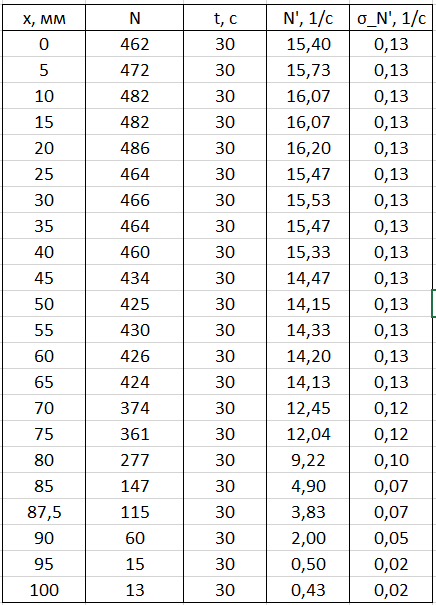
\includegraphics[width=0.5\linewidth]{images/table_1.png}
		\caption{Зависимость скорости счета частиц от расстояния между источником и счетчиком}
		\label{table 2}
	\end{figure}
\end{center}

\begin{center}    
    \begin{figure}[h!]
    \centering
		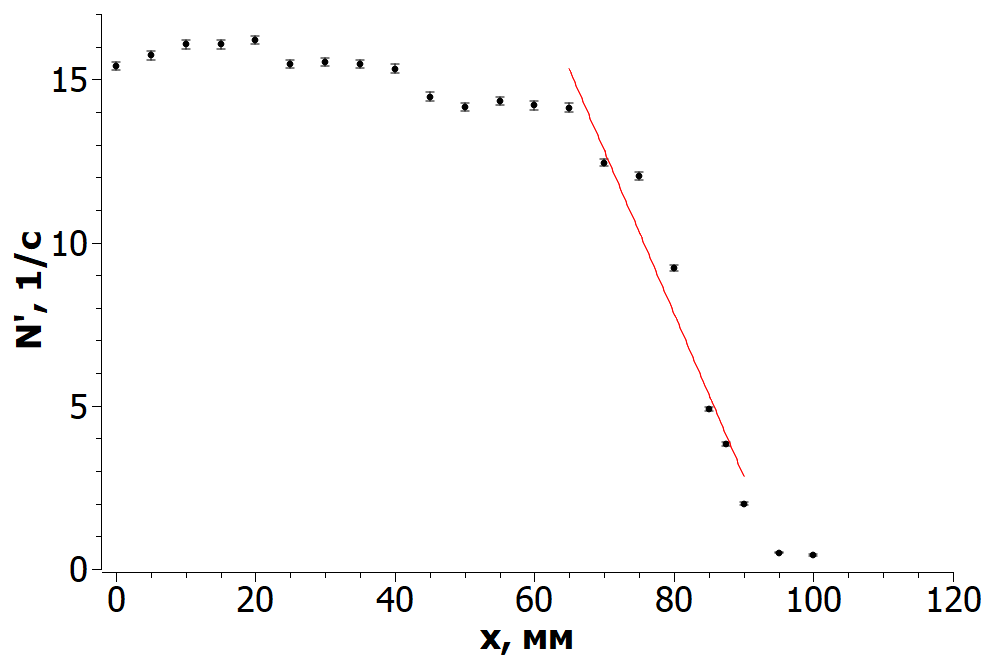
\includegraphics[width=0.9\linewidth]{images/graph_1.png}
		\caption{Зависимость скорости счета частиц от расстояния между источником и счетчиком}
		\label{table 2}
	\end{figure}
\end{center}

\item Получаем зависимость вида $y = ax + b$:

\begin{center}
\begin{tabular}{|c|c|c|}
\hline 
 & Значение & Погрешность \\ 
\hline 
a & -0.498 & 0.006 \\ 
b & 47.7 & 0.5 \\ 
\hline 
\end{tabular} 
\end{center}

	\item Экстраполируем полученую прямую до пересечения с осью абсцисс. Отсюда получаем экстраполированную длину пробега
		 
		 \begin{equation}\label{}
			 R_{\text{э}} = \dfrac{b}{a} \approx 95.4 \pm 1.5 \; мм \to R'_{\text{э}} = \rho R_{\text{э}} = (12,12 \pm 0,19)\cdot 10^{-3} \; \text{г}/\text{см}^2
		 \end{equation}	
		
	\item Энергию таких альфа-частицы можно оценить по эмпирической формуле 
		
		\begin{equation}\label{}
		R = 0,32 E^{3/2} \to E_{\text{э}} = \approx 11.28 \pm 0,18 \; МэВ
		\end{equation}		
		
\end{enumerate}
	
	\subsection{Ионизационная камера}

\begin{enumerate}	
	\item Включив питание установки, измерим при атмосферном давлении $P_a  = 745$ Торр (измеренном барометром) ток $I_a = 922$ пА. Температура $T = 295$ К. После этого откачаем воздух из камеры до давления порядка 10 Торр и снимем зависимость тока от давления.
	
	\item Погрешность давления оценим как цену деления --- $ \sigma_P = 5 $ Торр. Результаты измерения занесем в таблицу и построим график.

\begin{center}    
    \begin{figure}[h!]
    \centering
		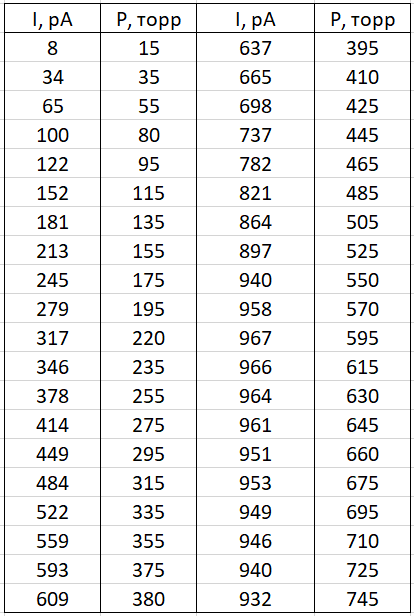
\includegraphics[width=0.5\linewidth]{images/table_2.png}
		\caption{Зависимость силы тока от давления в камере}
		\label{table 2}
	\end{figure}
\end{center}

	\item Построим две прямых, соответствующих линейным участкам графика. Результаты фита сведем в таблицу: 

\begin{center}    
    \begin{figure}[h!]
    \centering
		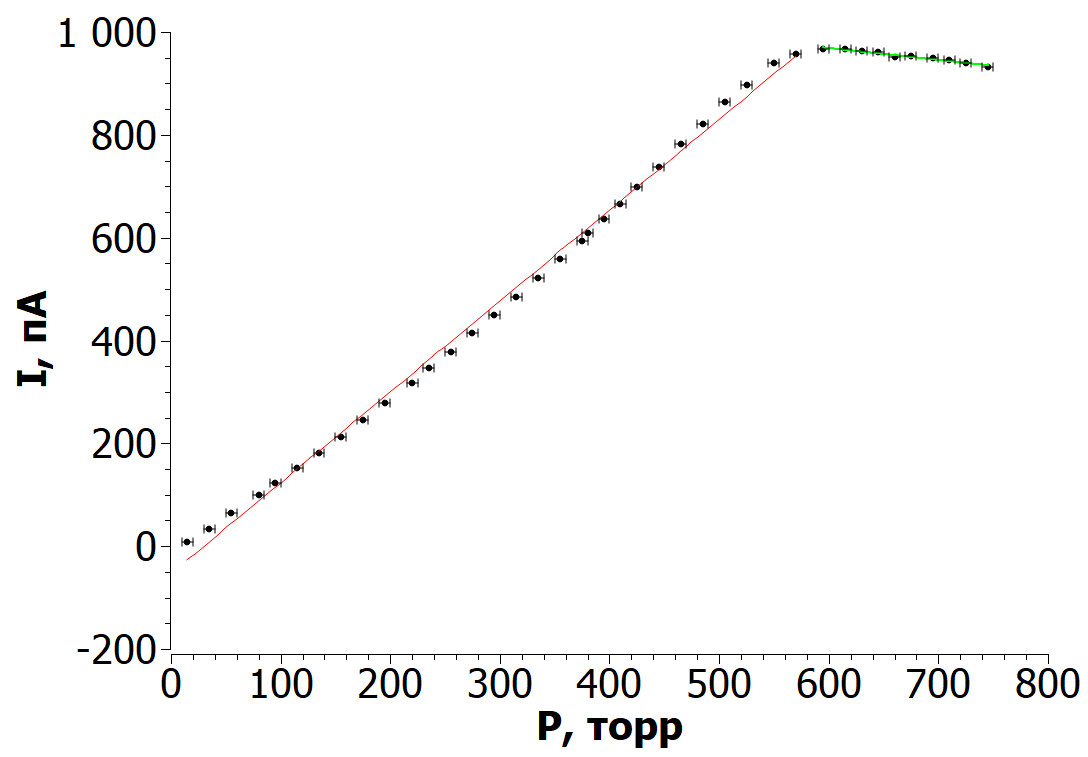
\includegraphics[width=0.9\linewidth]{images/graph_2.png}
		\caption{Зависимость тока от давления в ионизационной камере}
		\label{table 2}
	\end{figure}
\end{center}

	Результаты приближения вида $y = ax + b$ занесем в таблицу:

\begin{center}
\begin{tabular}{|c|c|c|}
\hline 
 & a & b \\ 
\hline 
$x \in [15; 570]$ & $1.76 \pm 0.02$ & $-53.4 \pm 6.4$ \\ 
\hline 
$x \in [595; 745]$ & $-0.231 \pm 0.019$ & $1107 \pm 12$ \\ 
\hline 
\end{tabular} 
\end{center}

	 \item Их пересечение дает нам значение 
	
	\begin{equation}\label{}
	P_0 = \dfrac{b_2 - b_1}{a_1 - a_2} \approx (582 \pm 85) \; \text{Торр} 
	\end{equation}
	
	Так как пробег $ R_l = 5 $ см задается размером камеры, приведем его к н.у.:
	
	\begin{equation}\label{}
\	R_{\text{э}} = R_l \dfrac{\rho}{\rho_0} = R_l \dfrac{P_0T}{PT_0} \approx (3,81 \pm 0,56) \; \text{см} \to R'_{\text{э}} \approx (4.84 \pm 0.71)\cdot 10^{-3} \; \text{г}/\text{см}^2
	\end{equation}
	
	Энергию такой альфа-частицы можно оценить по эмпирической формуле 
	
	\begin{equation}\label{}
	R = 0,32 E^{3/2} \to E_{\text{э}} = \left(  \dfrac{R}{0,32} \right)^{2/3} \approx 5.21 \pm 0.77 \; МэВ
	\end{equation}

\end{enumerate}

\section{Вывод}
	
	В работе был измерен пробег альфа-частиц от $ ^{239}  $Pu двумя способами :с помощью торцевого счетчика Гейгера и ионизационной камеры. По полученным данным была определена энергия альфа - частиц.

	
	При работе с ионизационной камерой пробег и энергия получились близкими к ожидаемым (из таблиц при $ E = 5 $ МэВ получаем $ R = 3,29 $ см для воздуха). При работе со счетчиком Гейгера значения пробега и энергий выше табличных. Это можно объяснить тем, что часть энергии альфа-частиц тратится на прохождение слюдяной пластинки, прикрывающей счетчик, и пленки, закрывающей источник. 
	
	Если плотность бумаги равна $ 1,2 \; \text{г}/\text{см}^3 $, следовательно, лист бумаги толщины $ l \geq R'/\rho =36, 6 $~мкм не пропустит альфа-частицы от $ ^{239}  $Pu.

\end{document}